\documentclass[tikz,border=8pt]{standalone}
\usepackage{tikz}
\usetikzlibrary{arrows.meta}
\begin{document}
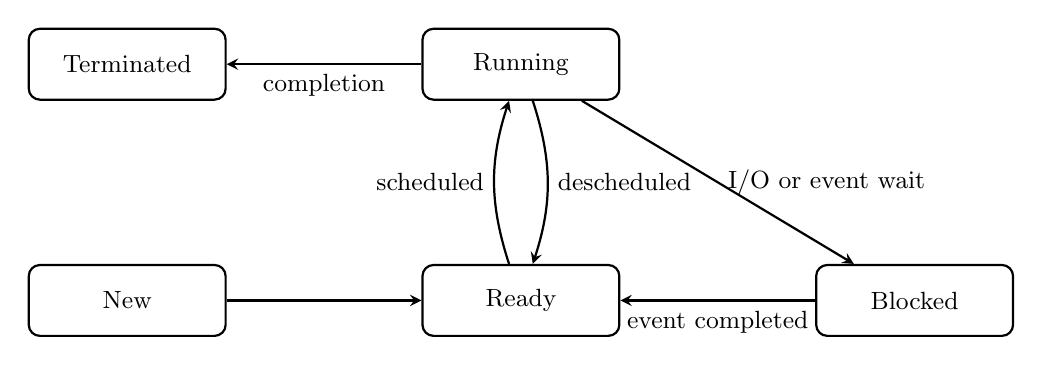
\begin{tikzpicture}[
        ->, >=stealth, thick,
        state/.style={draw, rounded corners, align=center,
                minimum width=2.5cm, minimum height=0.9cm},
        every node/.style={font=\small}
    ]
    \node[state] (new) at (0,-3) {New};
    \node[state] (ready) at (5,-3) {Ready};
    \node[state] (running) at (5,0) {Running};
    \node[state] (blocked) at (10,-3) {Blocked};
    \node[state] (terminated) at (0,0) {Terminated};

    \draw (new) -- node[above] {} (ready);
    \draw (ready) to[bend left=18] node[left] {scheduled} (running);
    \draw (running) -- node[right] {I/O or event wait} (blocked);
    \draw (blocked) -- node[below] {event completed} (ready);
    \draw (running) to[bend left=18] node[right] {descheduled} (ready);
    \draw (running) -- node[below] {completion} (terminated);
\end{tikzpicture}
\end{document}
